Die TEE zeichnet sich durch drei wesentliche Eigenschaften aus, die ihre Funktionalität und Sicherheit beschreiben. 
Sie gewährleistet (1) die Authentizität des ausgeführten Codes.
Ein wichtiger Aspekt dabei ist die Möglichkeit der Remote Attestation. Diese erlaubt es, die Authentizität des Codes aus der Ferne zu verifizieren. 
Die TEE sichert (2) die Integrität des Codes, indem sie gewährleistet, dass dieser nicht verändert wurde. Außerdem schützt sie (3) die Vertraulichkeit von Code, Daten und Laufzeitvariablen~\cite{Trusted}.

Aufgrund der Interaktion von Programmen innerhalb der TEE mit Programmen außerhalb kann die TEE auch als Kompartiment betrachtet werden. Diese Struktur  ermöglicht eine klare Trennung zwischen den unterschiedlichen Kompartimenten und ermöglicht so eine bessere Kontrolle über den Zugriff.

\subsection{Trusted Execution Environment}
Der genaue Aufbau und das Verhalten von TEEs variiert, lässt sich aber, wie in Abbildung~\ref{fig:TEE} zu sehen ist, im Allgemeinen in zwei Kategorien einteilen: (1) die Single-World-TEEs, die sich einen Adressraum mit dem unprivilegierten Host teilen, und (2) die Two-Worlds-TEEs, bei denen die CPU konzeptionell in eine normale und eine sichere Welt unterteilt ist~\cite{TEEPaper}.

\begin{figure}[h]
    \centering
    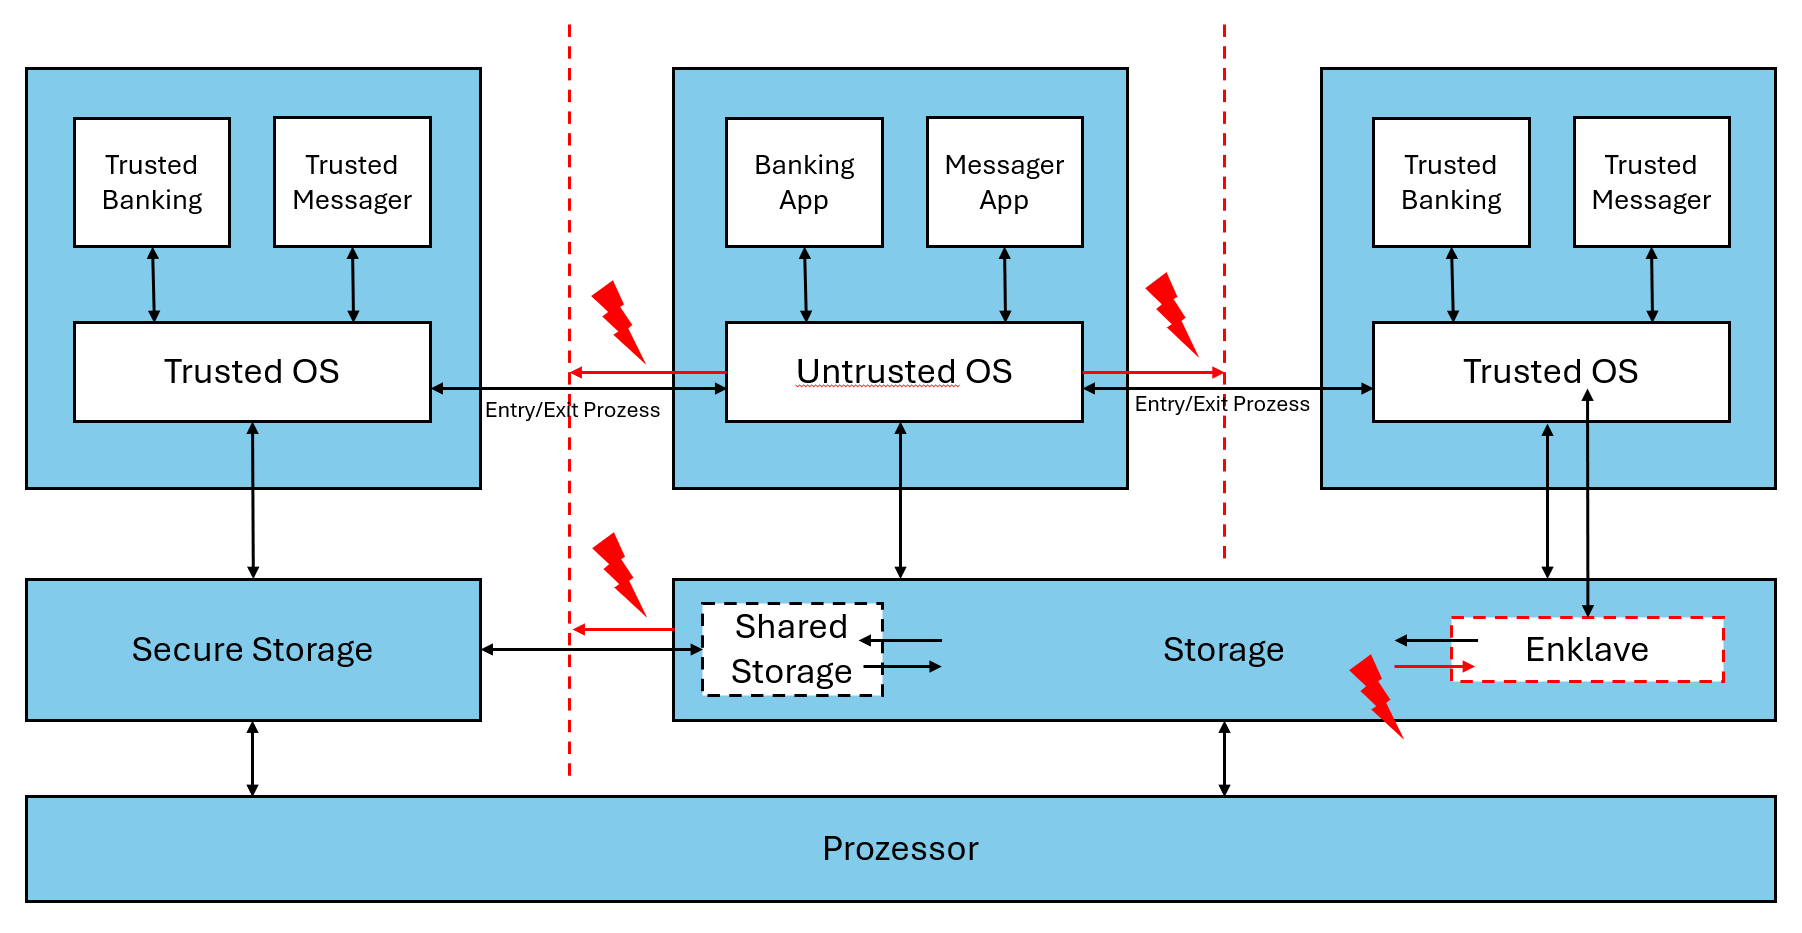
\includegraphics[width=\linewidth]{Grafiken/TEE-Grafik.png}
    \caption{Links der Aufbau einer TEE mit separatem Adressraum, rechts eine TEE mit geteilten Adressraum in Form einer Enklave im Adressraum des unsicheren Host.}
    \label{fig:TEE}
\end{figure}

In der ersten Kategorie hat nur die Enklave selbst vollen Zugriff auf ihren Speicherplatz und kann die Daten im Klartext lesen. 
Eine Enklave ist ein isolierter Speicherbereich innerhalb einer TEE, der dazu dient, Code und Daten vor unautorisiertem Zugriff und Manipulation zu schützen.
Selbst privilegierte Benutzer und das Betriebssystem haben keinen Zugriff auf die innerhalb der Enklave gespeicherten Daten. 
Programme innerhalb der Enklave dürfen jedoch auch auf den Adressraum außerhalb der Enklave zugreifen. 
Diese Struktur ermöglicht einen besseren Datenaustausch, birgt jedoch das Risiko unsicherer Speicherzugriffe auf möglicherweise korrupte Daten, was potenziell zu Sicherheitslücken führen kann. Wie in Abbildung \ref{fig:TEE} dargestellt, können Prozesse der unsicheren Welt oder auch das Untrusted OS, nicht auf die Prozesse des Sicheren OS zugreifen. Auch das Lesen der Daten in der Enklave ist nicht möglich.

In der zweiten Kategorie ist der Adressraum strikt in zwei separate Bereiche unterteilt, wobei keiner der beiden Bereiche auf den jeweils anderen zugreifen kann. 
Der Datenaustausch zwischen diesen beiden Welten erfolgt über das Trusted Operating System (TOS). 
Da das TOS privilegierten Zugriff hat, kann es einen geteilten Adressraum einrichten, in dem Daten sicher ausgetauscht werden können. 
Diese Methode bietet eine stärkere Isolation und somit ein höheres Maß an Sicherheit, da direkte Speicherzugriffe zwischen der normalen und der sicheren Welt verhindert werden, jedoch auf Kosten der Datenübertragungsraten. Wie in Abbildung \ref{fig:TEE} zu sehen ist es nicht möglich die Daten oder Prozesse der sicheren Welt einzusehen.

In beiden Kategorien gewährleistet sowohl der Prozessor, dass extern kein Zugriff auf die Daten möglich ist als auch das TOS, dass der Code in der Enklave sicher ist. Das TOS übernimmt außerdem den Entry/Exit Prozess der TEE, in dem der Übergang zwischen der normalen und der sicheren Welt ausgeführt wird. 

Neben den Angriffen auf das Application Binary Interface (ABI), welche auf Schwachstellen beim Erstellen und Verlassen der TEE abzielen, gibt es auch Angriffe auf das Application Programming Interface (API), welche versuchen, Sicherheitslücken während der Laufzeit zu nutzen~\cite{TEEPaper}.

Das Angreifermodell ist ein weiterer Grundgedanke beim Entwurf einer TEE. Die TEE wird unter der Annahme entwickelt, dass sie in einem System ausgeführt wird, das als kompromittiert betrachtet wird und Angreifer die volle Kontrolle über sämtliche Hardware haben.


\subsection{Kompartimentierung}

Die Kompartimentierung ist ein Konzept, das darauf abzielt, ein Computersystem oder einzelne Anwendungen in separate Bereiche aufzuteilen und diese möglichst isoliert voneinander operieren zu lassen. Diese Praxis beruht auf den Prinzipien der Sandbox und der Safebox, die eine sicherere und stabilere Systemumgebung ermöglichen. Ein Kompartiment agiert als Safebox und behandelt alle anderen Programme als Sandbox. So wird kein Zugriff auf die eigenen Daten erlaubt.

Eine Sandbox ist, wie in Abbildung~\ref{fig:Sandbox} dargestellt, eine isolierte Ausführungsumgebung, in der ein Programm ausgeführt wird, welches keinen Zugriff auf Daten anderer Programme hat. Die Applikation in der Sandbox kann, wenn überhaupt, nur über klar definierte APIs auf andere Programme oder Funktionen zugreifen, während anderen Applikationen vollen Zugriff gewährt wird.
Dies gewährleistet nicht nur die Sicherheit sensibler Informationen, sondern verhindert auch die Übernahme von Daten oder die Beeinflussung des Programmes durch potenziell kompromittierte Softwareteile. 
Ein bekanntes Beispiel dafür ist eine Virtuelle Maschine (VM). Diese wird in einer isolierten Umgebung ausgeführt und hat keinen Zugriff auf jegliche Daten außerhalb der Sandbox.

\begin{figure}[h]
    \centering
    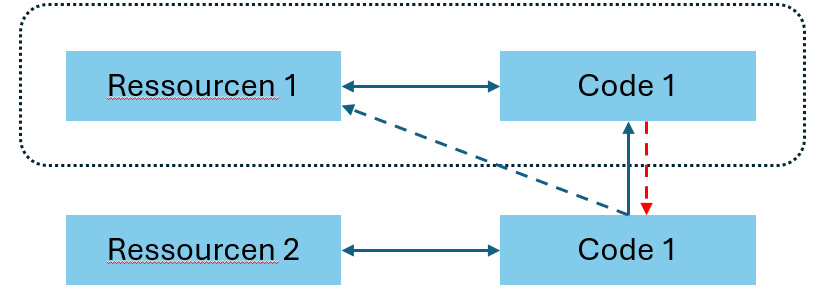
\includegraphics[width=0.67\linewidth]{Grafiken/Sandbox.png}
    \caption{Aufbau einer Sandbox: Applikationen in der Sandbox können nur über klar definierte APIs auf andere Programme zugreifen.}
    \label{fig:Sandbox}
\end{figure}

Im Gegensatz dazu dient die Safebox, in Abbildung~\ref{fig:Safebox} dargestellt, dem Schutz der eignen Daten. Dies wird ermöglicht, indem nur privilegierten Prozessen Zugriff auf die Daten gestattet wird. Diese Zugangskontrolle verhindert den Zugriff auf Daten eines anderen Kompartiments. Andere Kompartimente können nur über eine klare Schnittstelle Daten übertragen, während die Programme innerhalb vollen Zugriff haben. 
Dies spiegelt genau die Funktionsweise einer Enklave wider, in der Programme innerhalb vollen Zugriff haben, deren Daten aber für Programme aus der unsicheren Welt nicht lesbar sind.
\begin{figure}[h]
    \centering
    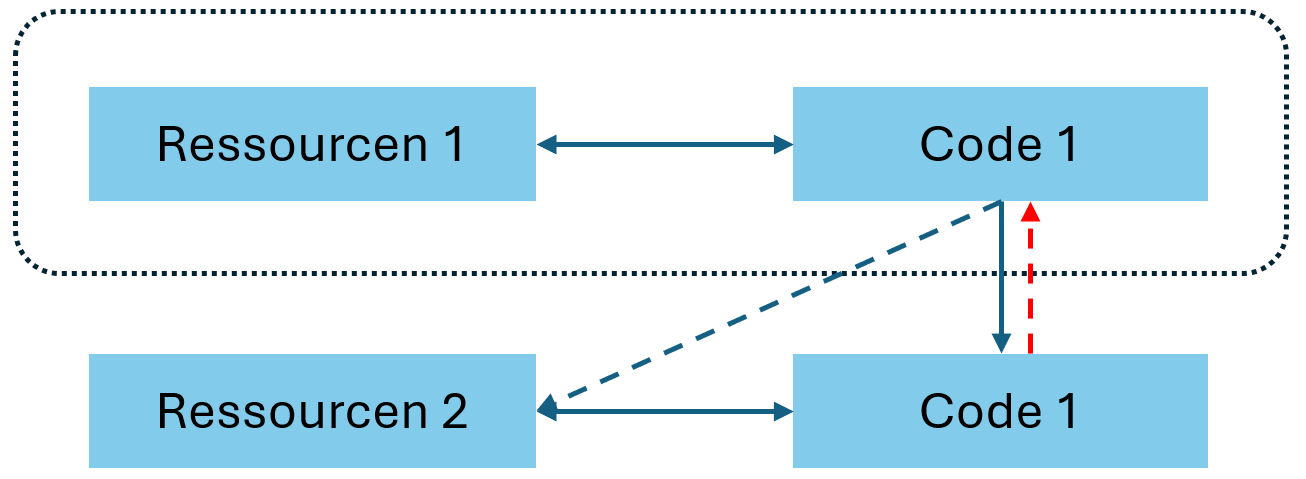
\includegraphics[width=0.67\linewidth]{Grafiken/Safebox.png}
    \caption{Aufbau einer Safebox: Applikationen außerhalb der Safebox können nur über eine klar definierte API auf Code innerhalb zugreifen.}
    \label{fig:Safebox}
\end{figure}

Das Initialisieren eines Kompartiments lässt sich in 3 Stufen unterteilen. Zunächst erfolgt (1) die Identifizierung, bei der festgelegt wird, an welcher Stelle das Programm logisch gut unterteilt werden kann und wie feingranular diese Unterteilung sein soll.
Anschließend wird (2) die Durchsetzung der Grenzen vorgenommen, indem die Programme logisch voneinander getrennt und ausschließlich über eine API zur Kommunikation zugelassen werden. 
In der letzten Stufe werden (3) diese Grenzen weiter verhärtet. Hierbei werden die API weiter definiert, wie z. B. die Rückgabewerte und Pointer.

Wie in Abbildung~\ref{fig:Kompartiment} dargestellt, können Applikationen in verschiedenen Kompartimenten nur über eine klar definierte API untereinander Daten austauschen und haben keinen Zugriff auf andere Informationen.

\begin{figure}[h]
    \centering
    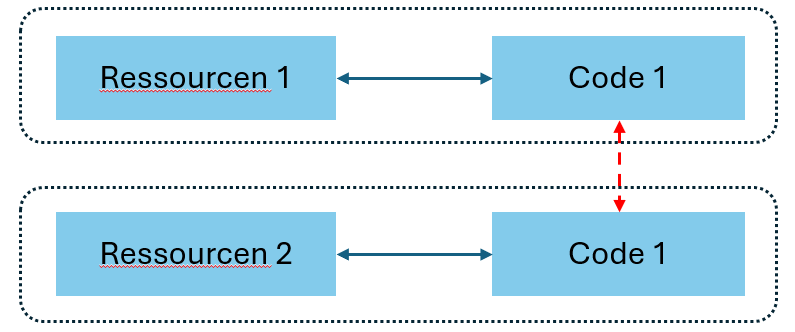
\includegraphics[width=0.67\linewidth]{Grafiken/Kompartiment.png}
    \caption{Aufbau von Kompartimenten: Applikationen in verschiedenen Kompartimenten können nur über eine klar definierte API Datein austauschen.}
    \label{fig:Kompartiment}
\end{figure}

